% =====================================================================================
% REVISIÓN 2  -  Propuesta de solución
% Escribe tu texto FUERA de los recuadros \begin{guia} ... \end{guia}.
% =====================================================================================

\section{Propuesta de solución} \label{sec:propuesta} % audit:req=propuesta_solucion

\begin{guia}[Guía: Propuesta de solución (Revisión 2)]
\textbf{¿Para qué sirve?} Explica \emph{qué vas a hacer exactamente y cómo resuelve el problema}, antes de entrar a los
detalles de construcción (Revisión 3).

\textbf{Debe responder:}
\begin{itemize}[nosep,leftmargin=*]
  \item ¿En qué consiste la solución, a grandes rasgos? Incluye un diagrama general (arquitectura, flujo del proceso o
        esquema del método).
  \item \emph{Proyecto de sistema:} ¿cuáles son los requisitos funcionales (qué hará) y no funcionales (rendimiento,
        seguridad, usabilidad)? ¿quiénes son los usuarios y qué roles tienen?
  \item \emph{Proyecto de investigación:} ¿cuál es la hipótesis o pregunta de investigación? ¿qué enfoque o algoritmo
        propones y en qué se diferencia de lo existente?
  \item ¿Qué tecnologías, herramientas y metodología de trabajo usarás y por qué (frente a las alternativas)?
  \item ¿Cómo atiende la propuesta cada objetivo específico? (una tabla ``objetivo $\rightarrow$ componente de la solución''
        es muy útil).
  \item ¿Cuál es el plan de trabajo y el cronograma del cuatrimestre?
  \item ¿Cómo sabrás que funcionó? (criterios de aceptación o métricas de éxito).
\end{itemize}

\textbf{Organización sugerida:} \verb|\subsection| para \emph{Descripción general}, \emph{Requisitos} (o \emph{Hipótesis y
enfoque}), \emph{Tecnologías y metodología} y \emph{Plan de trabajo}.

\textbf{Extensión mínima:} 150 palabras, además de diagramas y tablas.

\textbf{Errores frecuentes:} describir solo tecnologías sin explicar la solución; requisitos vagos (``el sistema será
rápido''); propuesta desconectada de los objetivos; cronograma sin fechas.

\textbf{Cómo se revisa:} coherencia con el problema y los objetivos, viabilidad en un cuatrimestre y claridad técnica.
\end{guia}

% >>> ESCRIBE AQUÍ la propuesta de solución (con una \subsection por apartado) <<<

\subsection{Descripción general de la solución}

La solución consiste en un sistema web institucional, de uso interno, que sustituye el circuito en papel por un flujo digital en el que cada documento recibe un identificador único al nacer y conserva, desde ese momento y hasta su resguardo, la constancia de todos los movimientos de que fue objeto. No se trata de digitalizar el formato de solicitud, sino de trasladar al sistema el control del proceso: el documento existe para la institución únicamente cuando ha sido registrado, y cada cambio de situación queda asentado por el propio sistema sin depender de que alguien recuerde anotarlo.

El principio que ordena el diseño es que la bitácora es la única fuente de verdad sobre lo ocurrido. Los módulos no llevan contadores propios ni estadísticas paralelas: toda cifra que el sistema reporta se deriva de los asientos de la bitácora, de manera que el indicador y la evidencia que lo sustenta son el mismo dato. Esta decisión, discutida en la Sección~\ref{sec:marco_teorico} a propósito de la pista de auditoría, es la que permite afirmar que lo reportado es comprobable.

La arquitectura se organiza en tres capas, como muestra la Figura~\ref{fig:arquitectura}. La estación de trabajo del usuario accede por navegador a través de un proxy inverso que termina el cifrado TLS; la capa de aplicación, alojada en el entorno virtualizado, concentra los módulos funcionales y el servicio transversal de bitácora; y la capa de persistencia separa deliberadamente la base de datos, que guarda metadatos y asientos, del acervo documental, que guarda los archivos fuera de la raíz pública del servidor y bajo nombres opacos. La separación no es cosmética: impide que un archivo sea alcanzable por una dirección adivinable y obliga a que toda entrega de documento pase por la verificación de permisos.

\begin{figure}[H]
  \centering
  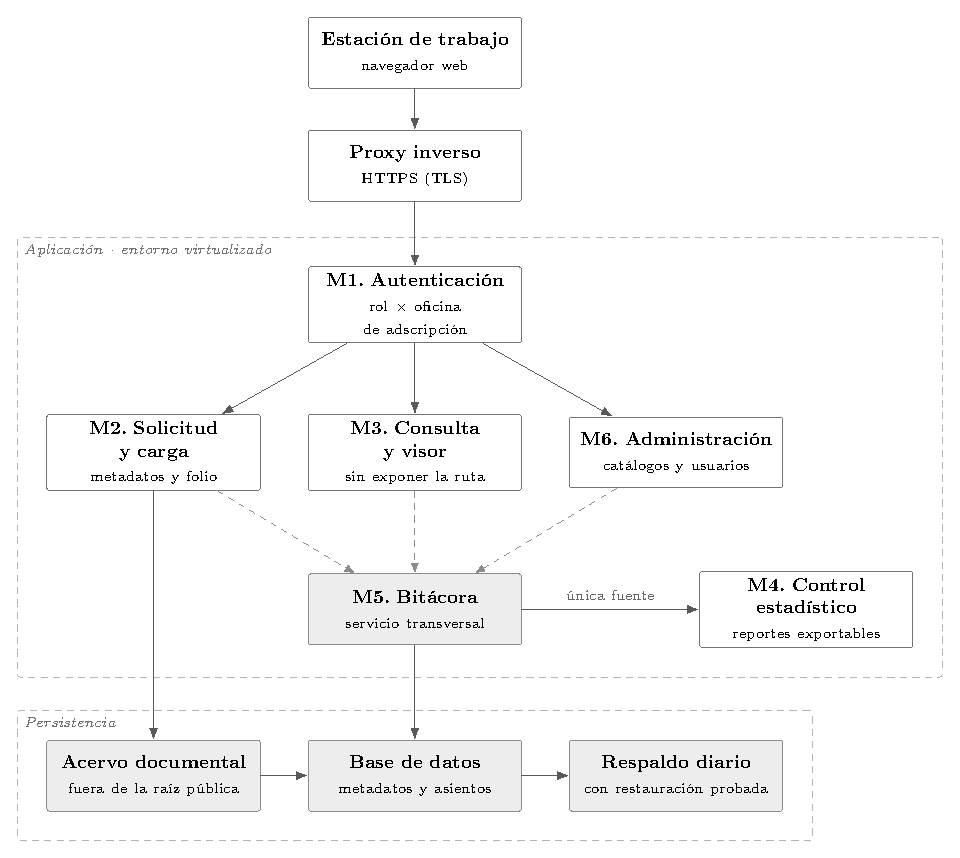
\includegraphics[width=0.78\textwidth]{img/arquitectura.pdf}
  \caption{Arquitectura general del sistema. El módulo de bitácora opera como servicio transversal y constituye la única fuente de la que se deriva el control estadístico.}
  \label{fig:arquitectura}
\end{figure}

El proceso que el sistema gobierna se muestra en la Figura~\ref{fig:flujo}. Una solicitud recorre cinco etapas —registro, carga, turnado, acuse y resguardo— y a cada una corresponde un estado explícito del expediente. La cancelación es el único camino alterno y exige motivo asentado. En todas las transiciones, incluida la cancelación, el servicio de bitácora escribe quién actuó, cuándo y sobre qué folio, y de ese conjunto de asientos se obtiene después el control estadístico.

\begin{figure}[H]
  \centering
  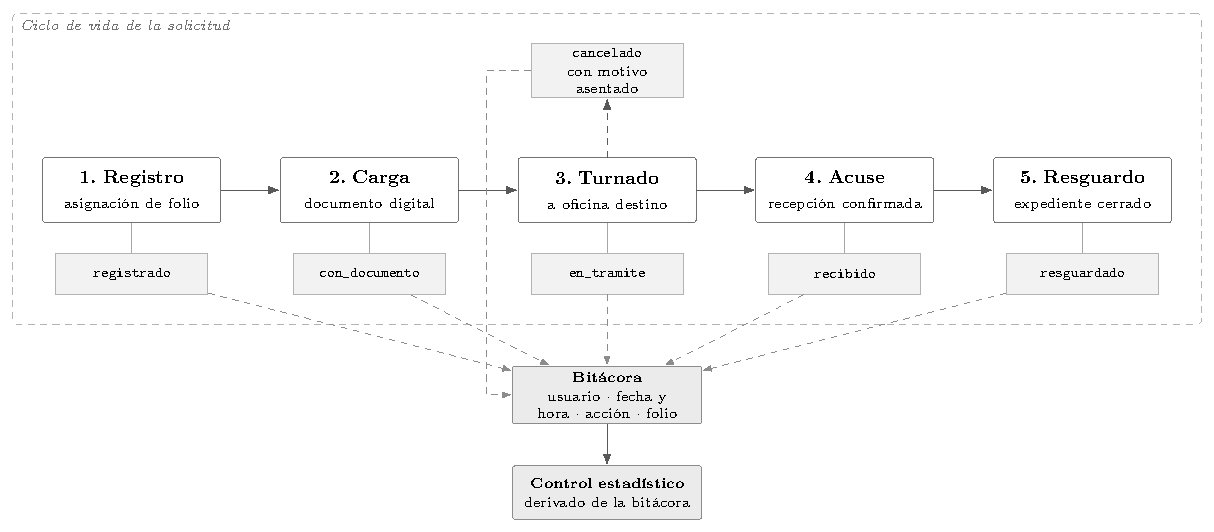
\includegraphics[width=\textwidth]{img/flujo_proceso.pdf}
  \caption{Ciclo de vida de una solicitud documental y puntos en los que el servicio de bitácora deja constancia del movimiento.}
  \label{fig:flujo}
\end{figure}

\subsection{Requerimientos funcionales}

Los requerimientos se enuncian de manera verificable, conforme al criterio de ISO/IEC/IEEE 29148 \cite{iso29148} expuesto en el marco teórico: cada enunciado debe poder confirmarse o refutarse mediante una prueba. Se agrupan por módulo y se identifican con la clave \texttt{RF} para su trazabilidad posterior.

Los que aquí se enuncian son los que definen la solución y delimitan su alcance, no el catálogo exhaustivo. El catálogo completo, con sus reglas de negocio y su matriz de trazabilidad, es el entregable del segundo objetivo específico y se valida con los responsables de cada oficina mediante acta firmada; lo que sigue es el subconjunto que permite juzgar si la propuesta resuelve el problema planteado.

\begin{description}[leftmargin=0pt,font=\bfseries,itemsep=0.6em,parsep=0pt]
  \item[M1. Autenticación y control de acceso]\leavevmode
  \begin{itemize}[nosep,leftmargin=1.4em,topsep=1pt]
    \item \textbf{RF-01.} El sistema autentica al usuario mediante credencial institucional y contraseña, y deniega el acceso tras cinco intentos fallidos consecutivos.
    \item \textbf{RF-02.} El sistema determina los permisos de cada usuario como la intersección de su rol y su oficina de adscripción, de modo que un capturista solo opera sobre los expedientes de su oficina.
    \item \textbf{RF-03.} El sistema cierra la sesión por inactividad y asienta en la bitácora tanto el inicio como el cierre de sesión.
  \end{itemize}

  \item[M2. Solicitud y carga de documentos]\leavevmode
  \begin{itemize}[nosep,leftmargin=1.4em,topsep=1pt]
    \item \textbf{RF-04.} El sistema asigna a cada solicitud un folio institucional único con la forma \texttt{IRCT-\textless oficina\textgreater-\textless año\textgreater-\textless consecutivo\textgreater}, irrepetible aun ante registros simultáneos.
    \item \textbf{RF-05.} El sistema exige los metadatos obligatorios que correspondan al tipo documental seleccionado y rechaza el registro incompleto.
    \item \textbf{RF-06.} El sistema admite archivos en los formatos y tamaños autorizados, calcula su huella criptográfica y los almacena fuera de la raíz pública con nombre opaco.
    \item \textbf{RF-07.} El sistema conserva las versiones anteriores de un documento sustituido junto con el motivo del cambio, sin eliminar el antecedente.
    \item \textbf{RF-08.} El sistema permite turnar un expediente a otra oficina y registrar el acuse de recepción por parte de la oficina destino.
  \end{itemize}

  \item[M3. Consulta y visualización]\leavevmode
  \begin{itemize}[nosep,leftmargin=1.4em,topsep=1pt]
    \item \textbf{RF-09.} El sistema localiza expedientes por folio, asunto, tipo documental, oficina y rango de fechas.
    \item \textbf{RF-10.} El sistema presenta el documento en un visor dentro del navegador, sin exponer la ruta del archivo. La visualización en línea es el modo predeterminado; la descarga se habilita solo a los perfiles autorizados y exige asentar el motivo.
    \item \textbf{RF-11.} El sistema muestra el historial completo de movimientos de un expediente a los perfiles autorizados.
  \end{itemize}

  \item[M4. Control estadístico]\leavevmode
  \begin{itemize}[nosep,leftmargin=1.4em,topsep=1pt]
    \item \textbf{RF-12.} El sistema calcula, a partir de la bitácora, el volumen documental y su distribución por usuario, oficina, tipo documental y periodo, así como el tiempo transcurrido entre etapas.
    \item \textbf{RF-13.} El sistema identifica los expedientes que exceden el plazo definido para su etapa actual.
    \item \textbf{RF-14.} El sistema exporta los reportes en formato de hoja de cálculo y en PDF, indicando el periodo y los filtros aplicados.
  \end{itemize}

  \item[M5. Bitácora y auditoría]\leavevmode
  \begin{itemize}[nosep,leftmargin=1.4em,topsep=1pt]
    \item \textbf{RF-15.} El sistema asienta en la bitácora todo acceso, alta, modificación, consulta, turnado, acuse, cancelación y exportación, con usuario, fecha y hora, acción, folio y dirección de origen.
    \item \textbf{RF-16.} El sistema impide la modificación y el borrado de los asientos de bitácora, incluso para el perfil administrador.
  \end{itemize}

  \item[M6. Administración]\leavevmode
  \begin{itemize}[nosep,leftmargin=1.4em,topsep=1pt]
    \item \textbf{RF-17.} El sistema permite administrar usuarios, roles, oficinas, tipos documentales y plazos sin intervención del desarrollador.
    \item \textbf{RF-18.} El sistema deshabilita usuarios sin eliminarlos, a fin de preservar la integridad de los asientos históricos.
  \end{itemize}
\end{description}

El marco teórico sostiene, siguiendo a ISO/IEC/IEEE 29148, que ningún requerimiento debe existir sin un hallazgo que lo motive y ningún hallazgo debe quedar sin requerimiento que lo atienda. La Tabla~\ref{tab:trazabilidad} comprueba esa condición sobre los cinco puntos de pérdida de trazabilidad enunciados en el planteamiento del problema.

\begin{table}[H]
  \centering
  \small
  \renewcommand{\arraystretch}{1.3}
  \caption{Trazabilidad entre los puntos de pérdida identificados en el planteamiento del problema y los requerimientos que los atienden.}
  \label{tab:trazabilidad}
  \begin{tabularx}{\textwidth}{@{}>{\raggedright\arraybackslash}p{3.3cm}>{\raggedright\arraybackslash}X>{\raggedright\arraybackslash}p{3.1cm}@{}}
    \toprule
    \textbf{Punto de pérdida} & \textbf{Cómo lo atiende el sistema} & \textbf{Requerimientos} \\
    \midrule
    Tránsito invisible & Estado explícito del expediente en cada etapa, con fecha de turnado y de acuse, e historial consultable & RF-08, RF-11 \\
    Ausencia de identificador único & Folio institucional generado por el sistema, con clave de oficina y consecutivo anual irrepetible & RF-04 \\
    Registro heterogéneo & Metadatos obligatorios definidos por tipo documental y configurables desde la administración & RF-05, RF-17 \\
    Consulta sin huella & Asiento en bitácora de toda consulta y descarga, con garantía de inalterabilidad en el motor & RF-15, RF-16 \\
    Sustitución sin versionado & Conservación de las versiones anteriores con el motivo del cambio, sin borrado del antecedente & RF-07 \\
    \bottomrule
  \end{tabularx}
\end{table}

\subsection{Requerimientos no funcionales}

Los requerimientos no funcionales se formulan sobre las características del modelo de calidad ISO/IEC 25010 \cite{iso25010} y se acompañan del valor que permite comprobarlos, para evitar enunciados como ``el sistema será rápido''.

Los valores de la Tabla~\ref{tab:rnf} son metas de diseño derivadas del volumen documental y del número de usuarios que el Instituto maneja hoy en las oficinas participantes. Se consignan desde ahora porque un requerimiento no funcional sin cifra no es verificable, y se confirman o se ajustan con el Instituto durante la fase de especificación, en la misma acta en que se valida el catálogo funcional. Lo que no admite ajuste es su carácter medible: la cifra podrá cambiar, pero cada enunciado conservará una prueba que lo decida.

\begin{table}[H]
  \centering
  \small
  \renewcommand{\arraystretch}{1.3}
  \caption{Requerimientos no funcionales, característica de calidad asociada y criterio de verificación.}
  \label{tab:rnf}
  \begin{tabularx}{\textwidth}{@{}>{\raggedright\arraybackslash}p{2.1cm}>{\raggedright\arraybackslash}p{2.9cm}>{\raggedright\arraybackslash}X@{}}
    \toprule
    \textbf{Clave} & \textbf{Característica} & \textbf{Enunciado verificable} \\
    \midrule
    RNF-01 & Eficiencia de desempeño & Las consultas por folio responden en menos de tres segundos con un acervo de cincuenta mil expedientes y veinte usuarios concurrentes. \\
    RNF-02 & Seguridad & El tránsito se cifra con TLS; las contraseñas se almacenan con función de derivación con sal; el sistema se prueba contra las categorías vigentes de OWASP \cite{owasp2021}. \\
    RNF-03 & Seguridad & Ningún archivo es alcanzable por dirección directa: toda entrega pasa por verificación de rol y oficina. \\
    RNF-04 & Fiabilidad & El respaldo de base de datos y acervo se ejecuta diariamente y su restauración se prueba al menos una vez antes de la liberación. \\
    RNF-05 & Usabilidad & Un capturista registra una solicitud completa en no más de ocho campos y tres pantallas, tras una capacitación de treinta minutos. \\
    RNF-06 & Compatibilidad & La interfaz es responsiva y opera en las versiones vigentes de los navegadores instalados en el Instituto, con comportamiento verificado desde 1\,024 píxeles de ancho. \\
    RNF-07 & Mantenibilidad & El código se versiona en repositorio con historial de cambios y se entrega con manual técnico que documenta despliegue y configuración. \\
    RNF-08 & Portabilidad & La solución se despliega mediante contenedores, de modo que el entorno local de desarrollo y el entorno del Instituto sean equivalentes. \\
    \bottomrule
  \end{tabularx}
\end{table}

\subsection{Usuarios y roles}

El sistema reconoce seis perfiles. El permiso efectivo de cada usuario no resulta únicamente de su rol, sino de la intersección entre ese rol y la oficina a la que está adscrito, conforme al principio de privilegio mínimo expuesto en el marco teórico.

\begin{table}[H]
  \centering
  \small
  \renewcommand{\arraystretch}{1.3}
  \caption{Perfiles de usuario, responsabilidad y ámbito de actuación dentro del sistema.}
  \label{tab:roles}
  \begin{tabularx}{\textwidth}{@{}>{\raggedright\arraybackslash}p{3.0cm}>{\raggedright\arraybackslash}X>{\raggedright\arraybackslash}p{3.1cm}@{}}
    \toprule
    \textbf{Perfil} & \textbf{Qué hace} & \textbf{Ámbito} \\
    \midrule
    Administrador del sistema & Gestiona usuarios, roles, catálogos y parámetros; no opera expedientes ni altera la bitácora & Toda la institución \\
    Responsable de oficina & Autoriza, turna y da por recibidos los expedientes de su oficina & Su oficina \\
    Capturista & Registra solicitudes, carga documentos y captura metadatos & Su oficina \\
    Consultante & Localiza y visualiza expedientes conforme a su autorización & Su oficina \\
    Auditor & Revisa la bitácora y el historial de movimientos; no modifica información & Toda la institución, solo lectura \\
    Directivo & Consulta indicadores y reportes agregados & Toda la institución, solo agregados \\
    \bottomrule
  \end{tabularx}
\end{table}

\subsection{Tecnologías y metodología}

La selección de tecnologías responde a tres condiciones del contexto: que la solución deba operar en la infraestructura del Instituto sin costo de licenciamiento adicional, que deba poder ser mantenida por su área técnica una vez concluida la estadía, y que deba construirse y liberarse dentro de un cuatrimestre.

\begin{description}[leftmargin=0pt,font=\bfseries,itemsep=0.6em,parsep=0pt]
  \item[Lenguaje y marco de trabajo]\leavevmode
  \begin{itemize}[nosep,leftmargin=1.4em,topsep=1pt]
    \item Se emplea PHP con el marco de trabajo Laravel \cite{laraveldocs}. Frente a la alternativa de construir sobre un marco de otro ecosistema, Laravel ofrece resueltos de origen los mecanismos que el proyecto necesita —autenticación, control de acceso por políticas, migraciones de base de datos, validación en servidor y protección contra las vulnerabilidades más frecuentes—, lo que concentra el esfuerzo del cuatrimestre en la lógica del proceso documental y no en la infraestructura del sistema.
    \item La interfaz se construye con el motor de plantillas del propio marco, sin incorporar una biblioteca de interfaz reactiva. La decisión es deliberada: el sistema es de formularios y listados, no de interacción intensiva, y evitar una segunda tecnología reduce la superficie que el área técnica del Instituto deberá mantener.
  \end{itemize}

  \item[Persistencia y almacenamiento]\leavevmode
  \begin{itemize}[nosep,leftmargin=1.4em,topsep=1pt]
    \item La base de datos es MariaDB, por su compatibilidad con la infraestructura existente y por soportar las transacciones ACID que exige la asignación de folio sin colisiones.
    \item Los archivos no se guardan en la base de datos sino en un directorio dedicado fuera de la raíz pública, referenciados desde la base por su identificador y huella criptográfica. Así, el respaldo de la base permanece ligero y la integridad del archivo es comprobable.
  \end{itemize}

  \item[Entorno y despliegue]\leavevmode
  \begin{itemize}[nosep,leftmargin=1.4em,topsep=1pt]
    \item El entorno se define mediante contenedores, lo que permite desarrollar localmente en una réplica del entorno destino y migrar sin cambios en el código. Esta decisión mitiga directamente la limitación señalada en la Sección~\ref{subsec:limitaciones}: si la asignación del entorno virtualizado del Instituto se retrasa, el desarrollo continúa sin detenerse.
    \item El código se versiona en repositorio con historial de cambios, lo que constituye además la evidencia del cuarto objetivo específico.
  \end{itemize}
\end{description}

En cuanto a la metodología, el proyecto se conduce con un enfoque iterativo e incremental basado en Scrum \cite{scrumguide2020}. La razón de preferirlo a un modelo secuencial es la expuesta en la Sección~\ref{subsec:mt_ingenieria}: los requerimientos del flujo documental se precisan al confrontarlos con quienes lo ejecutan, y la fecha de término es inamovible. Un modelo en cascada atiende mal la primera condición y un enfoque ágil sin fases ni hitos verificables atiende mal la segunda.

La adaptación a un proyecto de un solo desarrollador es la anticipada en el marco teórico. El asesor empresarial asume el rol de dueño del producto, pues es quien decide qué se construye y en qué orden; los roles de equipo de desarrollo y de maestro Scrum se concentran en el estadista; y la reunión diaria, que carece de sentido en un equipo de una persona, se sustituye por una bitácora de avance, impedimentos y decisiones, que sirve además como evidencia del seguimiento. Se conservan sin modificación los sprints de dos semanas, con un incremento funcional demostrable al cierre de cada uno ante el asesor empresarial, la pila de producto priorizada y las reuniones de planeación, revisión y retrospectiva, que son los elementos que dan ritmo y control al avance.

\subsection{Correspondencia entre objetivos y componentes}

La Tabla~\ref{tab:objetivo_componente} relaciona cada objetivo específico enunciado en la Sección~\ref{subsec:objetivos_especificos} con el componente de la propuesta que lo atiende y con el entregable que permitirá verificarlo, a fin de hacer explícito que ningún objetivo queda sin correspondencia.

\begin{table}[H]
  \centering
  \small
  \renewcommand{\arraystretch}{1.3}
  \caption{Correspondencia entre cada objetivo específico, el componente de la solución que lo atiende y su entregable verificable.}
  \label{tab:objetivo_componente}
  \begin{tabularx}{\textwidth}{@{}>{\raggedright\arraybackslash}p{2.9cm}>{\raggedright\arraybackslash}X>{\raggedright\arraybackslash}X@{}}
    \toprule
    \textbf{Objetivo} & \textbf{Componente de la solución} & \textbf{Entregable verificable} \\
    \midrule
    1. Diagnosticar & Caracterización del flujo documental vigente y de sus puntos de pérdida de trazabilidad & Documento de diagnóstico y flujo documental caracterizado \\
    2. Especificar & Catálogo de requerimientos funcionales y no funcionales, Tabla~\ref{tab:rnf} & Especificación de requerimientos y actas de validación \\
    3. Diseñar & Arquitectura de tres capas, Figura~\ref{fig:arquitectura}; modelo de datos; prototipos de interfaz & Diagrama entidad-relación, documento de arquitectura y prototipos validados \\
    4. Implementar & Entorno virtualizado contenedorizado, base de datos, red, usuarios y repositorio & Entorno operando y repositorio con historial \\
    5. Desarrollar & Módulos M1 a M6, incluidos el servicio transversal de bitácora y la administración de catálogos & Módulos en operación y pruebas por historia de usuario \\
    6. Liberar y transferir & Plan de pruebas funcionales, de integración y de seguridad; respaldo y monitoreo; manuales y capacitación & Evidencias de prueba, acta de liberación y lista de asistencia \\
    \bottomrule
  \end{tabularx}
\end{table}

\subsection{Plan de trabajo y cronograma}

El proyecto se desarrolla en catorce semanas, del lunes 31 de agosto al viernes 4 de diciembre de 2026, con una carga de 600 horas. La Tabla~\ref{tab:cronograma} distribuye el trabajo en seis fases alineadas con los objetivos específicos.

Dos criterios ordenan esa distribución. El primero es que las seis semanas centrales se reservan íntegras al desarrollo, de modo que los tres sprints de dos semanas comprometidos en la metodología quepan completos y ninguno deba recortarse sobre la marcha. El segundo es que las dos primeras semanas y las dos últimas no se asignan a construcción: las iniciales corresponden al diagnóstico y las finales a pruebas, liberación y transferencia. Reservarlas de antemano responde al riesgo más frecuente en proyectos de este tipo, que es que el desarrollo se extienda hasta absorber el tiempo de las pruebas y de la capacitación, y que el sistema termine entregado pero no adoptado.

La fase de especificación ocupa una sola semana porque no comienza de cero: la elicitación de requerimientos se inicia durante el diagnóstico, al conversar con los responsables de cada oficina sobre el proceso vigente, de manera que esa semana se dedica a formalizar, depurar y validar lo ya recogido.

\begin{table}[H]
  \centering
  \small
  \renewcommand{\arraystretch}{1.3}
  \caption{Cronograma del proyecto por fases, semanas de ejecución y resultado comprometido.}
  \label{tab:cronograma}
  \begin{tabularx}{\textwidth}{@{}>{\raggedright\arraybackslash}p{3.3cm}>{\raggedright\arraybackslash}p{2.6cm}>{\raggedright\arraybackslash}X@{}}
    \toprule
    \textbf{Fase} & \textbf{Semanas} & \textbf{Resultado comprometido} \\
    \midrule
    1. Diagnóstico & 1 y 2 \newline (31 ago -- 11 sep) & Caracterización del proceso vigente y de sus puntos de pérdida de trazabilidad \\
    2. Especificación y planeación & 3 \newline (14 -- 18 sep) & Requerimientos validados, alcance confirmado y pila de producto priorizada \\
    3. Diseño & 4 y 5 \newline (21 sep -- 2 oct) & Arquitectura, modelo de datos y prototipos de interfaz validados con usuarios \\
    4. Implementación del entorno & 6 \newline (5 -- 9 oct) & Entorno virtualizado y de desarrollo operando, con repositorio activo \\
    5. Desarrollo por incrementos & 7 a 12 \newline (12 oct -- 20 nov) & Sprint 1 (sem.\ 7 y 8): M1 y M5 \newline Sprint 2 (sem.\ 9 y 10): M2 y M6 \newline Sprint 3 (sem.\ 11 y 12): M3 y M4 \\
    6. Pruebas, liberación y transferencia & 13 y 14 \newline (23 nov -- 4 dic) & Pruebas ejecutadas, sistema en producción con respaldo, manuales entregados, personal capacitado y reporte final integrado \\
    \bottomrule
  \end{tabularx}
\end{table}

El módulo de bitácora se construye en el primer incremento y no al final, pese a no ser el más visible. La razón es que los módulos posteriores escriben en él: si se dejara para el cierre, los movimientos de los módulos ya construidos no habrían quedado registrados y el control estadístico carecería de datos sobre los cuales operar.

\subsection{Criterios de aceptación}

Se considerará que la propuesta cumplió su propósito si al cierre de la estadía se satisfacen los siguientes criterios, verificables sobre el sistema en operación y no sobre declaraciones:

\begin{enumerate}[nosep,leftmargin=*]
  \item \textbf{Trazabilidad completa.} Para cualquier expediente tomado al azar, el sistema reconstruye la secuencia íntegra de sus movimientos indicando usuario, fecha y hora de cada uno, sin omisiones.
  \item \textbf{Unicidad del folio.} Una prueba de registro concurrente no produce folios repetidos ni huecos atribuibles a error.
  \item \textbf{Inalterabilidad de la bitácora.} Un intento deliberado de modificar o borrar un asiento, ejecutado con el perfil administrador, es rechazado por el sistema.
  \item \textbf{Correspondencia entre indicador y evidencia.} Toda cifra de un reporte estadístico puede desglosarse hasta los asientos de bitácora que la componen, y la suma coincide.
  \item \textbf{Control de acceso efectivo.} Un usuario adscrito a una oficina no logra visualizar ni descargar documentos de otra, incluso solicitando la dirección del archivo de manera directa.
  \item \textbf{Recuperabilidad.} La restauración del respaldo se ejecuta con éxito en un entorno limpio y el sistema queda operativo con la información íntegra.
  \item \textbf{Apropiación institucional.} El personal capacitado registra, turna y consulta expedientes sin asistencia del desarrollador, y el área técnica despliega el sistema siguiendo únicamente el manual técnico.
\end{enumerate}

Los cinco primeros criterios comprueban en operación lo que la Tabla~\ref{tab:trazabilidad} compromete en el catálogo de requerimientos: trazabilidad reconstruible, folio irrepetible, bitácora inalterable, indicadores que se desglosan hasta su evidencia y control de acceso efectivo. Los dos últimos aseguran que la solución sobreviva a la conclusión de la estadía, que es la condición que distingue un sistema entregado de un sistema adoptado.
